
First in this section the method for building the corpus is introduced. Then
a new web-based application for collaborative metaphor annotation and coding 
is introduced.  This tool allows for efficient export, including a data 
analysis pipeline API for custom Python applications.  
The methods for data export and analysis are demonstrated. Finally, the
statistical methods used for finding the phase transitions in figurative 
violence use are discussed.

\subsection{Corpus}
\label{subsec:Corpus}

The corpus a set of 607 transcripts from cable news shows aired from
September 1, 2016 to November 30, 2016 (inclusive). The transcripts were from
six shows from three networks, Fox News, MSNBC, and CNN. The shows were the
two most watched shows from each network for the month of
October, 2016 \cite{Katz2016}. The shows and their networks are listed in 
Table \ref{tab:shows}. 

\vspace{.2in}

\begin{table}[!htb]
  \centering
    \begin{tabular}{|c|c|}
      \hline
        Network & Programs \\
      \hline
      \multirow{2}{*}{Fox News} 
        & The O'Reilly Factor \\
        & The Kelly File \\
      \hline
      \multirow{2}{*}{MSNBC}
        & The Rachel Maddow Show \\
        & The Last Word with Lawrence O'Donnell \\
      \hline
      \multirow{2}{*}{CNN}
        & Anderson Cooper 360 \\
        & Erin Burnett OutFront \\
      \hline
    \end{tabular}
  \caption{List of shows used in corpus and their networks.}
  \label{tab:shows}
\end{table}

While the transcripts may be available on each network's website 
for each of the days in the study range, we don't depend on this.
Instead, we use the Internet Archive's (\url{http://archive.org}) 
TV News Archive, or TVNA for short (\url{http://archive.org/tv/details}).
There are several reasons that the TVNA is prefereable to scraping network
websites for transcripts.
First, there is no guarantee that everything said on the show
will be in the transcript. The transcripts used here are built from the
closed captioning recorded and stored in the TVNA. 
Second, the Internet Archive provides a stable, though hidden, API for 
programmatic access to the data stored there. Therefore, the software built
for corpus building does not have to scrape three websites, it only needs to
scrape one. Included with calls to the TVNA is a wealth of metadata on each
show including the original air date, run time, links back to the TVNA, and
clip download links. These are all used to build rich software for corpus
building and annotation as demonstrated below.


\subsubsection{iatv: open source tool for TVNA scraping}
\label{subsec:iatv}

To access the data on the TVNA, I developed a new, open-source 
software tool in the Python programming language called \textit{iatv}
\cite{Turner2016}. More details can be found on the GitHub repository page
at \url{http://github.com/mtpain/iatv}. But as a brief example, here is
how one would download all transcripts and the associated metadata from
all shows aired on Fox News in September, 2016

\begin{minted}[fontsize=\small]{python}
from iatv import search_items, download_all_transcripts

# search string cannot be empty so use 'I'; set rows=1000 to get all shows 
items = search_items('I', channel='FOXNEWSW', time='201609', rows=1000)

# filter out commercials
shows = [item for item in items if 'commercial' not in item]

# base_directory will be created or overwritten by default
download_all_transcripts(shows, base_directory='FOXNEWSW-Sep2016')
\end{minted}

Here is an example of the directory structure of \texttt{base\_directory}, which
has been set to \texttt{FOXNEWSW-Sep2016}.

{\small
\begin{verbatim} 
FOXNEWSW-Sep2016
|
+-FOXNEWSW_20160901_000000_The_OReilly_Factor
|   |
|   +-FOXNEWSW_20160901_000000_The_OReilly_Factor.cc5.srt
|   +-metadata.json
|   +-transcript.txt
|
+-FOXNEWSW_20160901_010000_The_Kelly_File
|   |
|   +-FOXNEWSW_20160901_010000_The_Kelly_File.cc5.srt
...
\end{verbatim}
}

\noindent
The \texttt{base\_directory} is populated with subdirectories named by the Internet
Archive's ID for the program. Within each of those subdirectories, there is
the raw \texttt{.srt} file, containing the SubRip-formatted captions 
\cite{Matroska2016}, a metadata file containing all metadata obtained from the
TVNA, and a text file of the transcript converted from the \texttt{.srt} using
\href{https://github.com/pbs/pycaption}{PBS's \texttt{pycaption} library} for Python
\cite{PBS2016}. This concludes the first step in the data acquisition and
processing pipeline, continued in the following sections.


\subsection{Metacorps: Web app and API for corpus annotation and analysis}
\label{sub:corpus-annotation}

Here we introduce the web application and underlying data model that allows us
to collaboratively code instances of metaphor using the \texttt{FOXNEWSW-Sep2016} as
an example. This process is implemented using the 
\href{http://github.com/mtpain/metacorps}{\texttt{metacorps} package} I developed
as part of this project \cite{Turner2017}. 
The package includes both the web application
front-end for collaborative metaphor coding and an API for building the 
specific datasets to be analyzed, including searching for relevant violent
words and phrases. 

In the first step of this process, we insert the data and metadata
acquired from the TVNA into a MongoDB database. No further pre-processing is done 
at this point.
Each subdirectory in the \texttt{FOXNEWSW-Sep2016} is considered an \texttt{IatvDocument},
which is represented as a Python class. All MongoDB collections are represented
as Python classes, using the \texttt{mongoengine} document-object mapping software
\cite{Mongoengine2017}. Then specific documents are selected for analysis, 
building a separate corpus under the collection \texttt{IatvCorpus}. 
An \texttt{IatvCorpus} is then used to build another collection type, a
\texttt{Project}. In building the project, a list of 
violent words or phrases that may be used figuratively must also be given.
Each of these words defines a \texttt{Facet}, and each \texttt{Facet} is comprised
of a list of \texttt{Instance} types. Instances are potential figurative uses
of violence. These instances are what are reviewed by annotaters.
In the web interface, the reviewers can read the paragraph in which the
instance occurred, mark whether the instance was indeed figurative, whether to
include it in the analysis (it may be figurative but not related to politics),
the underlying conceptual metaphor, the perpetrator and victim of violence,
the tense, and whether or not the construction is active or passive. A 
screenshot of the facet navigation page and the \textit{attack} instance
navigation and viewing page are shown in Figure \ref{fig:metacorps-screenshots}.

\begin{figure*}[t!]
    \centering
    \begin{subfigure}[b]{0.45\textwidth}
        \frame{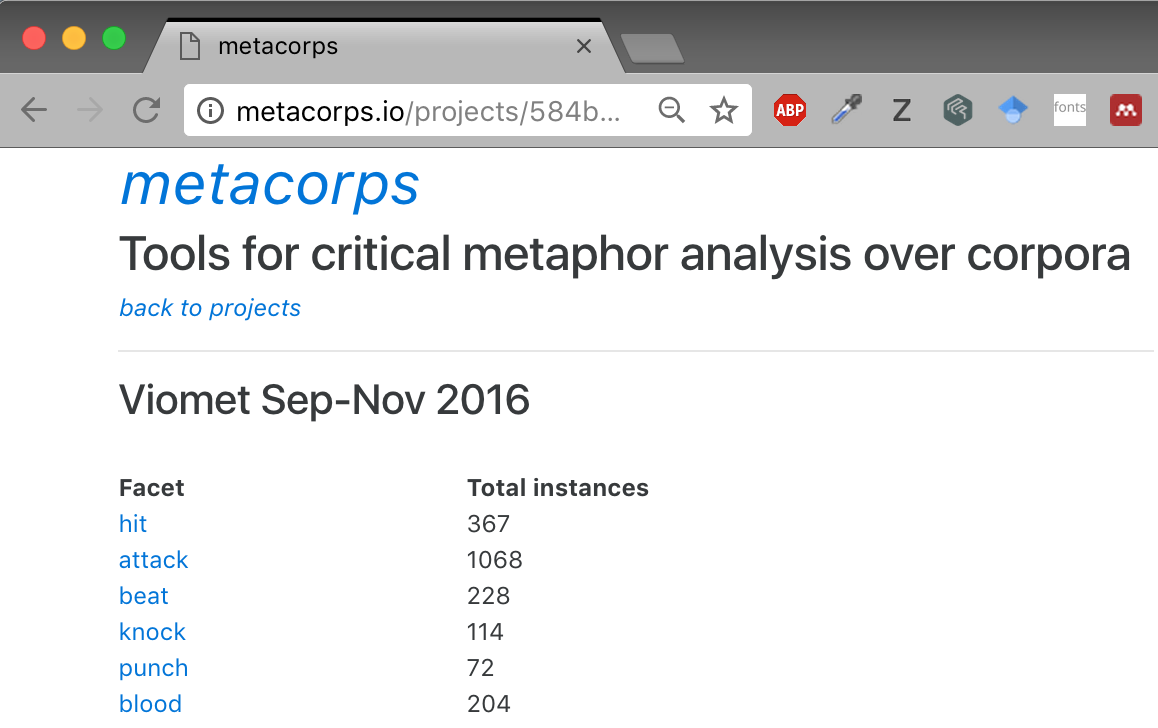
\includegraphics[width=\textwidth]{figures/facet-view.png}}
        \caption{Facet navigation}
    \end{subfigure}
    ~
    \begin{subfigure}[b]{0.45\textwidth}
            \frame{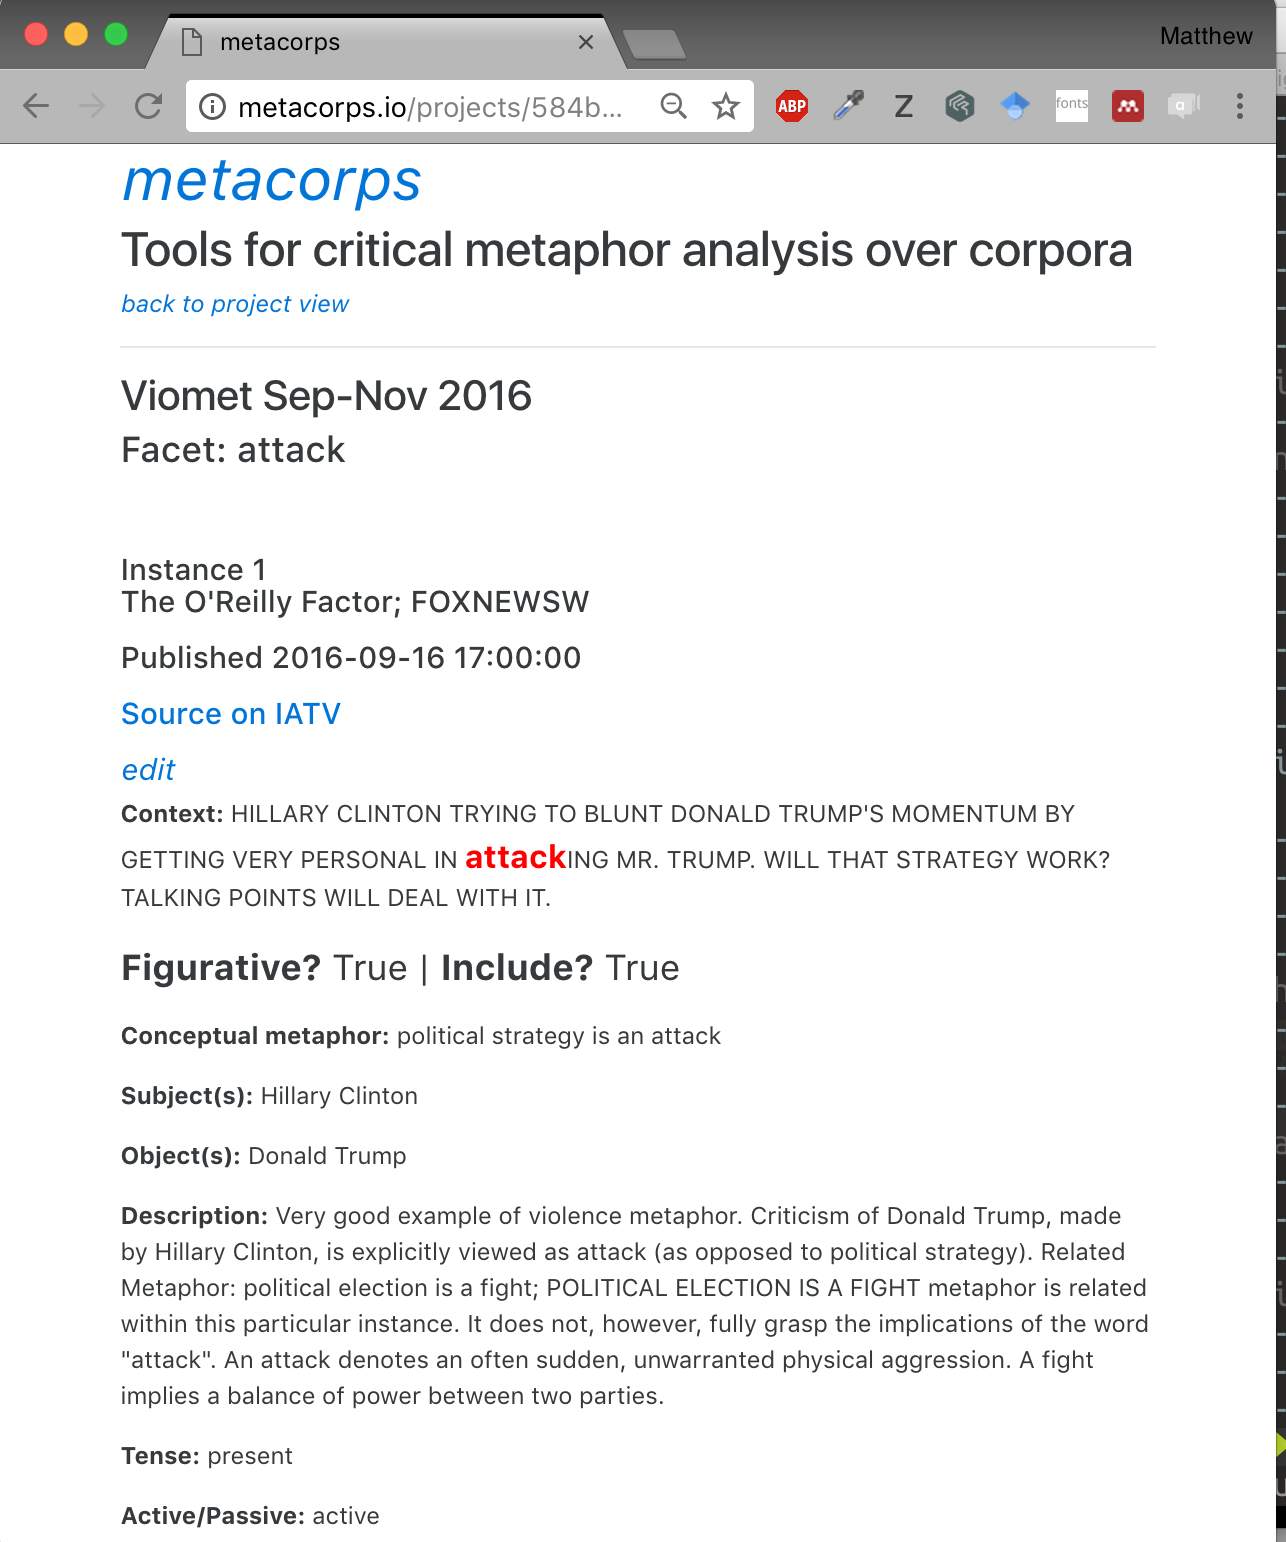
\includegraphics[width=\textwidth]{figures/instances-view.png}}
        \caption{Instance navigation for \textit{attack} facet}
    \end{subfigure}
    ~
    \caption{Screenshots of the Metacorps web app for metaphor annotation over
        corpora}
    \label{fig:metacorps-screenshots}
\end{figure*}

For this project, we had four people contributing to metaphor coding. In order
to keep track of progress and inform others of progress made, the Metacorps
web app includes a user log, shown in Figure \ref{fig:metacorps-home}. 
Once the coders finish annotating a project, it can be exported using an API
that's built-in to Metacorps itself. The user can export the annotations stored
in the database as CSV, or directly to a Pandas \texttt{DataFrame} object
\cite{McKinney2013} for interactive analysis or scripting.

\begin{figure}
    \centering
    \frame{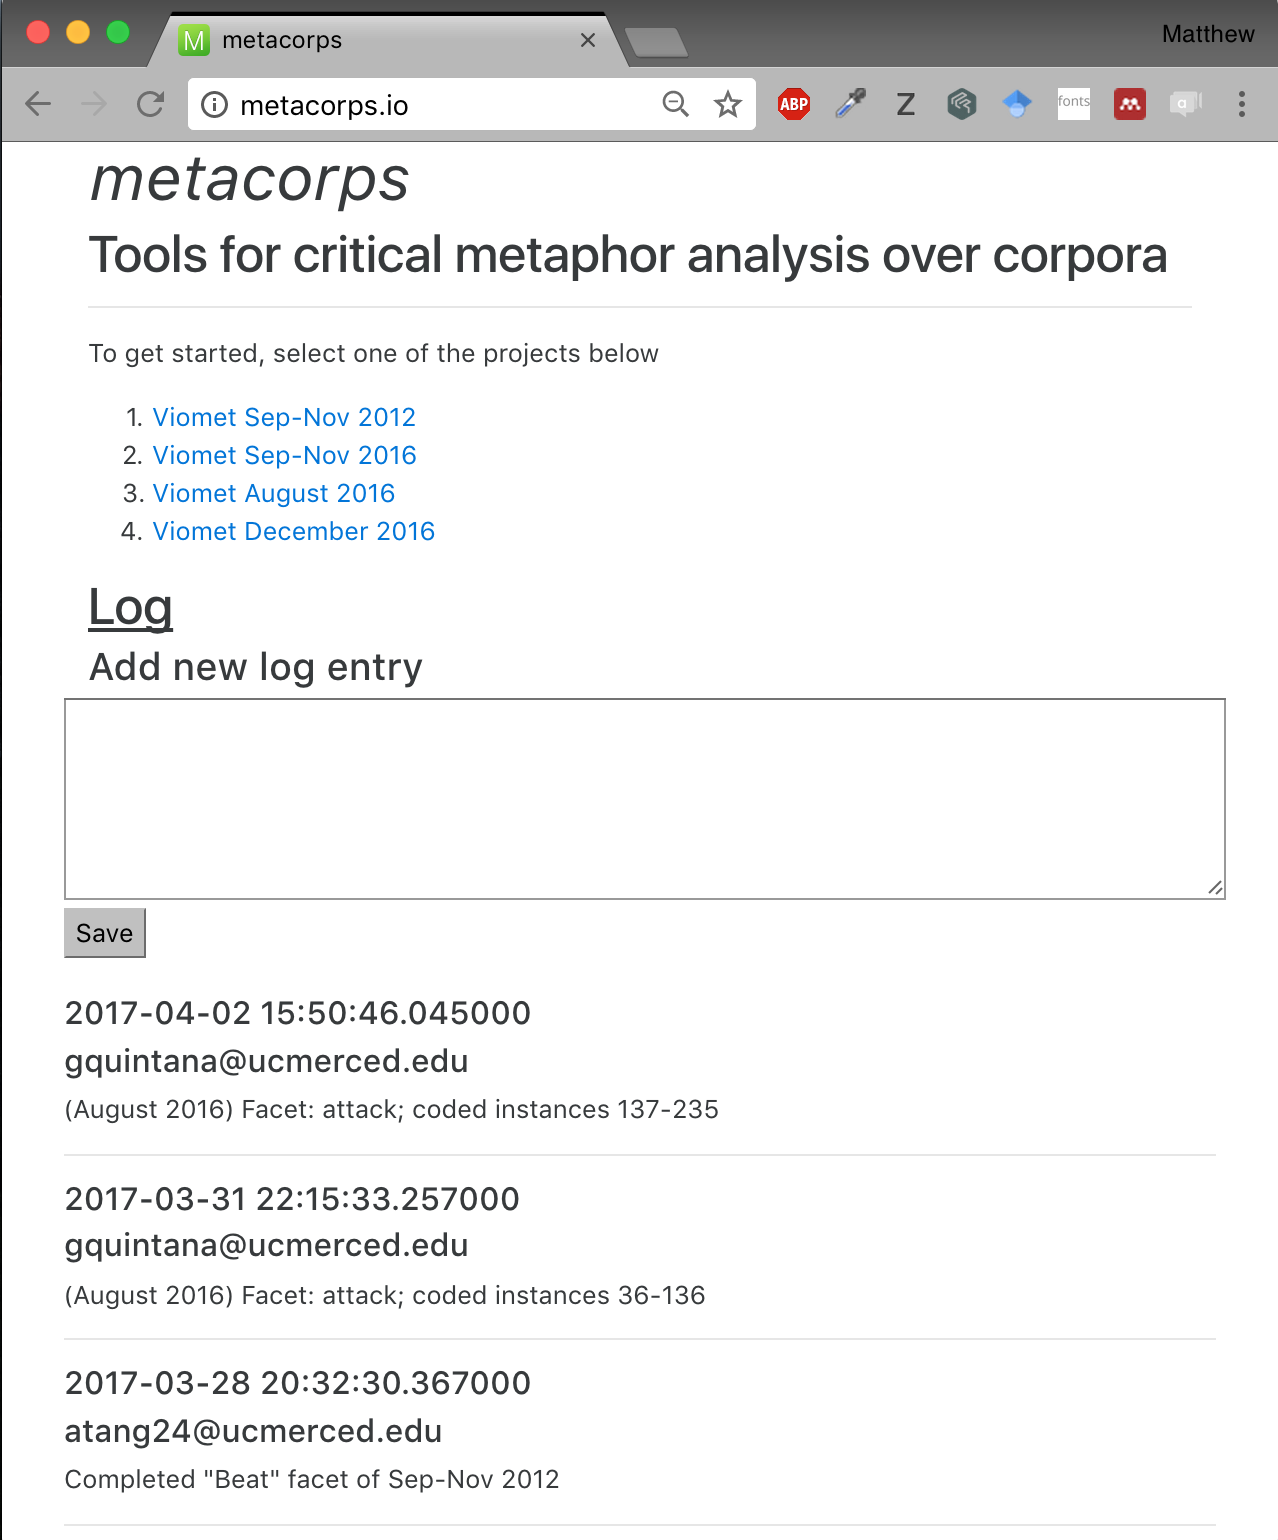
\includegraphics[width=0.75\textwidth]{figures/home-log.png}}
\caption{Home page of Metacorps web app. The metaphor coders use the log to
    inform others of progress. This is just the first step in making the
    app more social and collaborative.}
\label{fig:metacorps-home}
\end{figure}


\subsection{Statistical Analysis}
\label{sub:statistical-analysis}

To review, the goal of the statistical analysis is to determine if and when
phase transitions occur in the timeseries of uses of figurative violence
during the campaign. Preliminary analyses of the data revealed that by far
the most commonly used violent words in figurative violence constructions were
\textit{attack}, \textit{hit}, and \textit{beat}. In order to have higher 
counts and increase statistical power, usages were summed across all programs,
so each day we counted the total number of uses of each one of those words.
There is a sampling of this data table in Table \ref{tab:sample-data}. In 
order to assign phases one, two, and three to each row of this table, we
must first decide what candidate dates we should use for the first and
second phase transition. Part of the analysis is to find what the optimal 
dates are in terms of relative likelihood that the model with two particular
phase transition dates captures more information than any other candidate
model, including the null hypothesis, which is no dependence on phase.

\begin{table}[ht]
    \centering
    \begin{tabular}{|r|cc|}
        \hline
        date       &   facet    &  count     \\
        \hline
        2016-09-01 &     attack &    0     \\
        2016-09-02 &     hit    &    1     \\
        2016-09-03 &     hit    &    2     \\
        2016-09-04 &     beat   &    0     \\
        2016-09-05 &     beat   &    1     \\
        $\vdots$   &  $\vdots$  & $\vdots$ \\
    \end{tabular}
    \caption{Example first five rows of data used in statistical analysis to find
    phase transition before addition of phase}
    \label{tab:sample-data}
\end{table}

\begin{table}[ht]
    \centering
    \begin{tabular}{|r|ccc|}
        \hline
        date       &  phase  &   facet    &  count     \\
        \hline               
        2016-09-01 &    1    &     attack &    0     \\
        2016-09-02 &    1    &     hit    &    1     \\
        2016-09-03 &    1    &     hit    &    2     \\
        2016-09-04 &    1    &     beat   &    0     \\
        2016-09-05 &    1    &     beat   &    1     \\
        $\vdots$   & $\vdots$&  $\vdots$  & $\vdots$ \\
    \end{tabular}
    \caption{Example first five rows of data used in statistical analysis to find
    phase transition with addition of phase}
    \label{tab:sample-data-wphase}
\end{table}


To model the data we used general linear mixed models, 
with \texttt{phase} and \texttt{facet} 
being fixed effects. Because the data is count data, Poisson regression was
used. Because there could be fluctuations on any given day,
\texttt{date} is modeled as a random effect. Including random effects are
preferred to simply averaging as this results in less information loss
\cite{Winter2013, Burnham2011, Clark1973}. Model generation was done with
the \texttt{lme4} R package \cite{Bates2015} called seamlessly 
from Python using the \texttt{rpy2} package \cite{Gautier2017}. To summarize,
the two basic models tested are given in Table \ref{tab:models}. The 
theoretical and methodological innovation presented here is in building 
a series of 266 models with 14 candidate dates for the first phase transition
and 19 candidate dates for the second phase transition\footnote{More were
tested in preliminary stages; these correspond to a more specific region of
interest}. In this way, we are actually comparing 267 models: one is the null
hypothesis, that there is no improvement in model performance if we do not
include phase in the model. The 266 other models include phase in the model,
but the dates where we assign each phase are shifted. We performed preliminary
analysis to determine that it was significant to add \texttt{facet} as a 
fixed effect.

\begin{table}[ht]
    \centering
    \begin{tabular}{|r|c|}
        \hline
        description & formula \\
        \hline
        null model, facet only & \texttt{count $\sim$ facet + (1|date)} \\
        includes phase       & \texttt{count $\sim$ phase + facet + (1|date)} \\
        \hline
    \end{tabular}
    \caption{Two basic models considered for modeling figurative violence usage}
    \label{tab:models}
\end{table}

While one could use the chi-square test and significance values to evaluate
the improvement from one model to another, this becomes unwieldy and 
questionable when comparing 267 models. A more modern approach is to compare
the Akaike information criterion (AIC) of the models 
\cite{Akaike1974, Burnham2004, Burnham2011}. The AIC is a measure of 
information loss in a model. It has no meaning on its own, but it is instead
used to calculate the likelihood that another candidate model minimizes 
information loss better than the model with minimum AIC, or 
AIC$_{\mathrm{min}}$. Comparing model $i$ with AIC larger than 
the model that has minimum AIC, AIC$_{\mathrm{min}}$, 
the likelihood that model $i$ actually minimizes information loss is given by

\begin{equation}
    \mathcal{L}_i = \exp{\left(
      \frac{\mathrm{AIC}_{\mathrm{min}} - \mathrm{AIC}_{i}}{2} 
      \right)
      }
  \label{eq:relative-likelihood}
\end{equation}


In Section \ref{sec:Results}, Figures \ref{fig:AICs} and \ref{fig:relative-likelihoods}
show graphically the calculations of the AIC for all candidate phase
models and the relative likelihood of each candidate phase model, respectively.
